\chapter{GIỚI THIỆU ĐỀ TÀI}

\section{Bối cảnh và lý do chọn đề tài}

\textbf{Text-to-SQL} chuyển câu hỏi ngôn ngữ tự nhiên (NL question) thành truy vấn SQL thực thi được trên cơ sở dữ liệu quan hệ, đóng vai trò \emph{natural language interface to database} (NLIDB) \cite{ref1}. Theo \cite{ref1}, 51,52\% lập trình viên chuyên nghiệp dùng SQL nhưng chỉ khoảng 35,29\% được đào tạo bài bản, nên NLIDB giúp người không chuyên truy cập dữ liệu, đồng thời có thể giảm \emph{hallucination} của LLM nhờ nội dung thực từ CSDL. Nhóm chọn \cite{ref1} vì theo nhóm tác giả, đây là \emph{survey} đầu tiên về \emph{LLM-based Text-to-SQL}, có \emph{taxonomy} hệ thống.

\section{Định nghĩa bài toán và tiến trình phát triển}

Nhóm tác giả chia việc cài đặt \emph{LLM-based Text-to-SQL} thành ba khía cạnh: \emph{question under\-standing}, \emph{schema compre\-hension} và \emph{SQL gene\-ration}. Trong ICL (Eq. 3 \cite{ref1}), LLM \emph{\ensuremath{\pi}} với \emph{\ensuremath{\theta}} đóng băng sinh \emph{\ensuremath{\hat{Y}}} từ chỉ dẫn \emph{I}, câu hỏi \emph{Q} và \emph{schema} \emph{S} = \ensuremath{\langle}\emph{C}, \emph{T}, \emph{K}\ensuremath{\rangle} (cột, bảng, tri thức bổ sung như khóa ngoại):

\begin{equation}
\hat{Y} = \pi_{\theta}(I,Q,S)
\end{equation}

Text-to-SQL phát triển qua bốn giai đoạn (Hình 1.1) \cite{ref1}: (1) \textbf{Rule-based Methods} dùng luật, \emph{template} viết tay, đúng cú pháp nhưng kém với câu hỏi phức tạp, mơ hồ; (2) \textbf{Deep Learning-based Approaches} (\emph{sequence-to-sequence}, GNN) hay sinh SQL thiếu mệnh đề; (3) \textbf{PLM-based Implementation} (BERT, RoBERTa, RESDSQL \cite{ref2}) giảm mạnh khi sang miền mới; (4) \textbf{LLM-based Implementation} dùng \emph{prompt engineering} với LLM thương mại hoặc \emph{fine-tuning} LLM mã nguồn mở.

\begin{figure}[htbp]
\centering
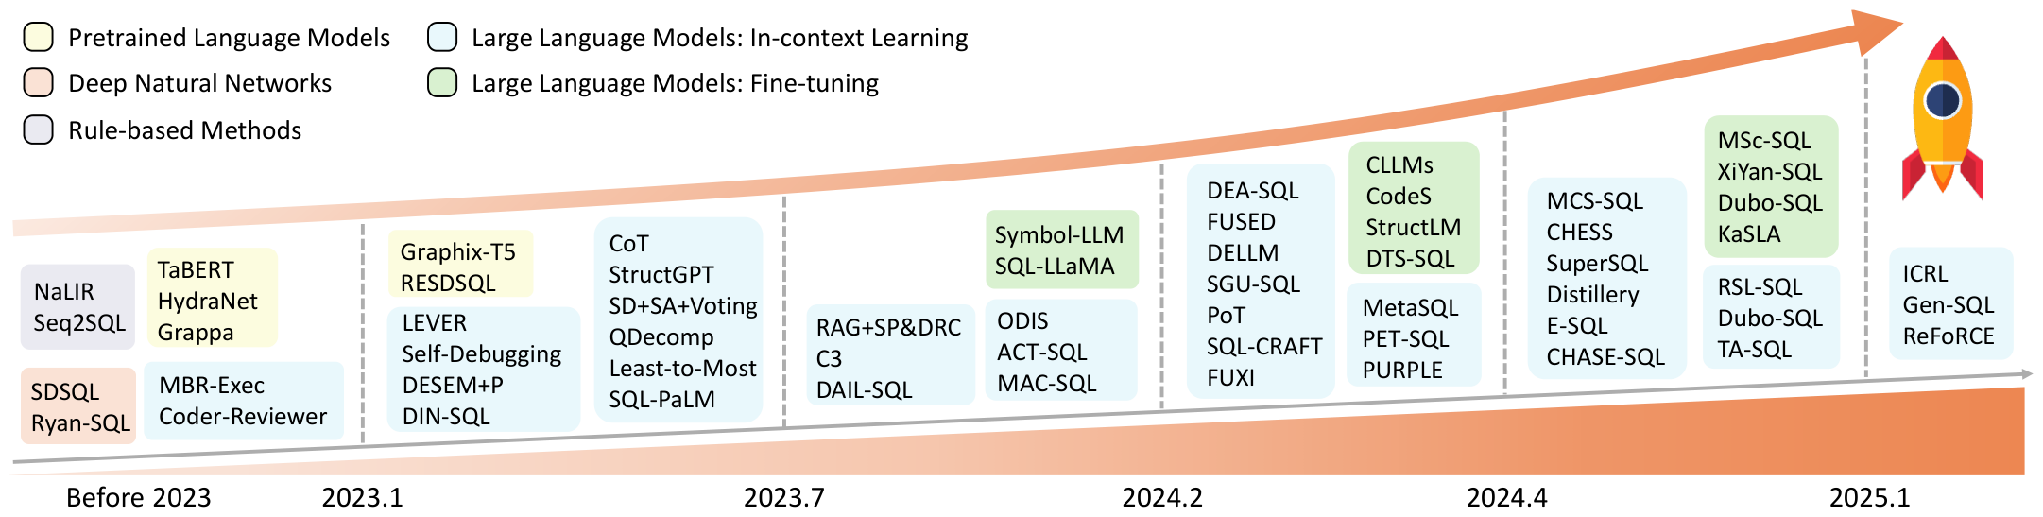
\includegraphics[width=\linewidth,height=0.68\textheight,keepaspectratio]{01-text-to-sql-evolution}
\caption{Tiến trình phát triển các nhánh phương pháp Text-to-SQL \cite{ref1}}\label{fig:01-text-to-sql-evolution}
\end{figure}

\section{Thách thức kỹ thuật và mục tiêu báo cáo}

Ở Mục II-A \cite{ref1}, nhóm tác giả nêu bốn thách thức: (1) \textbf{Linguistic Complexity and Ambiguity} (câu hỏi lồng, mơ hồ, nhiều cách diễn đạt); (2) \textbf{Schema Understanding and Representation} (\emph{schema} phức tạp, khác nhau theo miền); (3) \textbf{Rare and Complex SQL Operations} (truy vấn con lồng, \emph{outer join}, \emph{window function}); (4) \textbf{Cross-Domain Generalization} (kém đi khi sang miền khác). Mục V-A đối chiếu LLM với phương pháp truyền thống trên chính bốn thách thức này: LLM xử lý ngữ nghĩa tốt hơn nhưng tốn chi phí tính toán, thiếu minh bạch, có thể sinh SQL không hợp lệ và có nguy cơ \emph{overgeneralization}, nên nhóm tác giả gợi ý hướng \emph{hybrid} kết hợp cả hai. Hình 1.2 minh họa một ví dụ trên BIRD \cite{ref3}. Báo cáo hệ thống hóa \cite{ref1}, phân tích DIN-SQL \cite{ref4}, DAIL-SQL \cite{ref5}, MAC-SQL \cite{ref6} và đối sánh chúng cùng Codex MCP trên Spider dev.

\begin{figure}[htbp]
\centering
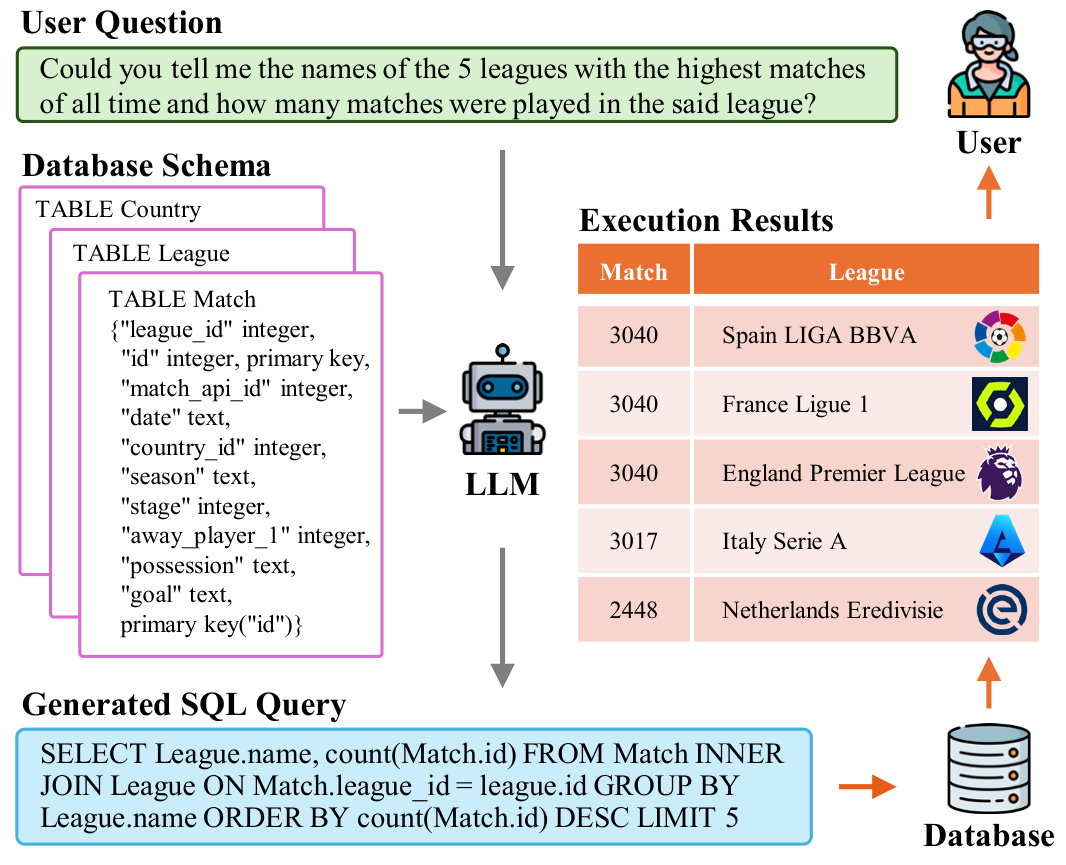
\includegraphics[width=\linewidth,height=0.68\textheight,keepaspectratio]{02-bird-example}
\caption{Minh họa quy trình LLM-based Text-to-SQL trên bộ dữ liệu BIRD \cite{ref1}}\label{fig:02-bird-example}
\end{figure}

